\documentclass[11pt]{article}

\usepackage[margin=0.78in]{geometry}

\usepackage[T1]{fontenc}

\usepackage[utf8]{inputenc}

\usepackage{lmodern}

\usepackage{microtype}

\usepackage{graphicx}

\usepackage{array,tabularx,longtable,booktabs}

\usepackage{enumitem}

\usepackage{hyperref}

\usepackage{xurl}

\usepackage{listings}

\usepackage{float}

\hypersetup{colorlinks=true,linkcolor=blue,citecolor=blue,urlcolor=blue}

\setlength{\parindent}{0pt}

\setlength{\parskip}{5pt}

\renewcommand{\arraystretch}{1.12}

\title{\Large\textbf{SpaceScope: A Big Data Analytics Framework for Historical Space Missions and Global Launch Trends}}

\author{
  \begin{tabular}{ccc}
    \textbf{Sakshi Naikwade} & \textbf{Sneha Supe} & \textbf{Pranav Mode} \\
    \multicolumn{3}{c}{\small Department of Computer Science and Engineering} \\
    \multicolumn{3}{c}{\small MIT World Peace University, Pune, India} \\[6pt]
    \multicolumn{3}{c}{\small \textbf{Project Guide:} Dr. Varsha Powar}
  \end{tabular}
}

\date{}

\begin{document}

\maketitle

\begin{center}\small Big Data Technologies (BDT) mini-project \textbullet{} October 2026 \textbullet{} Implementation \& Empirical Evaluation Results\end{center}

\begin{abstract}Historical records of orbital launch attempts are widely used to study reliability, national participation and industry growth, yet most published analyses concentrate on failure causes, selected countries or fixed periods, and rely on bespoke or specialist-database data preparation. This paper presents SpaceScope, an analytics framework for exploring historical space launch records and global launch trends. The framework ingests an openly available launch dataset (4,324 recorded launch attempts from 1957 to 2020), applies PySpark (DataFrame API and Spark SQL) for schema inspection, missing-value and duplicate analysis, date standardisation, categorical normalisation and derived-field construction, and then computes descriptive aggregates by year, organisation, launch vehicle, launch site and recorded outcome. Cleaned records and aggregates are stored in indexed MongoDB collections and served through a Python REST API. The analytical unit is the launch attempt, and the design deliberately separates launch attempts from payloads and missions, and an organisation's country from the country of the launch site. Empirical evaluation across the full historical dataset demonstrates effective preprocessing and distributed aggregation: exactly one business duplicate was eliminated (yielding 4,323 unique attempts), date and multi-part location parsing achieved 100\% validity, and 3,878 successful orbital flights were classified alongside 339 failures, 102 partial failures, and 4 prelaunch failures (89.71\% overall success rate). Temporal analysis captures the Cold War peak tempo (119 missions in 1971) alongside the modern commercial resurgence (117 missions in 2018). Stage-wise performance benchmarking confirms sub-second preprocessing (1.04~s) and sub-millisecond API query latencies (0.16~ms), providing a reproducible, descriptive, and extensible workflow for historical launch analytics.\end{abstract}

Keywords---Big Data Analytics, Space Missions, Historical Launch Data, Apache Spark, PySpark, MongoDB, Data Visualization.

\section{Introduction}

Since the first artificial satellite was placed in orbit in 1957, the record of human launch activity has grown from a handful of experimental flights into a continuous, international enterprise. Systematic studies of that record have a long history, and most of them are concerned with failure: early statistical summaries compared national failure rates and examined the first flights of new and modified vehicles [1], later work classified the causes of launch and spacecraft failures by subsystem [2], and more recent studies have analysed failures by mission phase and vehicle size over periods of one to two decades [3]. The reported tempo of launches has also changed substantially; one analysis of the period 2016--2021 notes an increase of roughly 70\% in launch attempts per year [3].

A second group of studies treats reliability as a statistical estimation problem. A NASA technical memorandum examines U.S. launch vehicles from 1980 to 2015 at the level of propulsion stages [4], while recent journal papers apply trend analysis, Bayesian estimation and Weibull modelling to launch vehicles from 2000 onwards [5] and to the launch programmes of five medium space powers [6]. Industry-oriented conference papers analyse the causes and consequences of failures over the last twenty years [7] and combine a review of the international launch industry with a probabilistic failure-assessment tool [8]. These contributions are valuable, but they share a common emphasis on failures and reliability, and the data preparation behind their figures is usually described only in summary.

Two open, versioned sources illustrate the diversity of publicly available launch records. The General Catalog of Artificial Space Objects (GCAT) maintained by McDowell provides launch lists together with organisation, launch-site and vehicle tables, and is distributed under a Creative Commons attribution licence [9]. Community-curated tabular datasets, such as the widely used ``All Space Missions from 1957'' collection hosted on Kaggle, offer a simpler schema in which each row describes one launch with fields such as the company, location, date, vehicle and mission status [10]. Such sources differ in granularity (launches, payloads, catalogued objects), in naming conventions for organisations and sites, in temporal coverage and in how outcomes are labelled. Analysing them consistently therefore requires explicit cleaning, integration and validation steps, a problem that has long been recognised in the data-quality literature [21].

Big Data technologies offer a standard vocabulary and toolset for this kind of work. The value chain of Big Data is commonly described as data generation, acquisition, storage and analysis [11]. MapReduce popularised a batch programming model for large clusters [12]; Apache Spark generalised it with resilient distributed datasets that support in-memory reuse of working sets and lineage-based fault tolerance [13], [14], and now offers a unified engine for batch, SQL and other workloads [15]. Spark SQL adds a DataFrame API and a relational optimiser on top of this engine [16]. For storage of heterogeneous, nested analytical outputs, document-oriented NoSQL stores such as MongoDB are a widely used option [19].

This paper proposes SpaceScope, a framework that connects these elements into a single, documented workflow for historical launch analytics: ingestion of an open launch dataset, PySpark-based preprocessing and aggregation, MongoDB storage of cleaned records and analytical summaries, and an interactive React dashboard served by a Python API. It is important to state the scope of this paper precisely. The work presented here is a proposed architecture and evaluation design; no experimental results are claimed. The main contributions are (i) a launch-attempt-centred analytical model that separates attempts, payloads, missions, organisation country and launch-site country; (ii) a reproducible preprocessing and aggregation pipeline specification; (iii) a MongoDB data model for analytical outputs; (iv) a dashboard design grounded in an established taxonomy of interactive analysis tasks [22]; and (v) an evaluation protocol covering data quality, metric correctness, processing time, query latency and scaling, designed so that performance claims are made only on the basis of controlled measurements.

\section{Related Work and Literature Review}

This review is based on a targeted, non-systematic search of publisher, institutional and repository sources (Springer, ACM, USENIX, IEEE-indexed records, the NASA Technical Reports Server and the International Astronautical Federation digital library). Peer-reviewed journal and conference papers are preferred; datasets, official documentation and institutional reports are identified as such. For several conference papers only abstracts or excerpts were accessible, and this is recorded in Appendix D. Table I summarises each source.

\subsection{Historical launch analysis, reliability and industry trends}

The earliest study in the reviewed set analyses worldwide launch failures from 1980 to early 2002, provides a statistical summary, compares national failure rates, and separately examines the first launches of new or newly modified vehicles [1]. Its contribution is a cross-national comparison and a set of recommendations for the launch industry; its limitations for the present purpose are its early end date and its presentation as a fixed analysis rather than a reusable data pipeline. A study of orbital carrier-rocket and spacecraft failures for 2000--2009 reports launch statistics and examines the faults behind failures, with particular attention to computer-based control systems and their hardware and software components [2]. Its single-decade scope and its focus on fault causes mean that it illustrates decade-level launch statistics but not long-run, multi-dimensional trend exploration.

Ayala Fernández et al. investigate launch failures between 2006 and 2021, together with post-mission disposal statistics [3]. Every failure recorded in launch logs was investigated and classified individually; 79 failures were analysed and five unconfirmed failures were excluded. Failures are classified by subsystem and mission phase, and the proportion occurring on first flights of a vehicle version is examined. The method is rigorous but depends on manual classification of a failure subset; the paper is nevertheless useful to SpaceScope because it makes explicit that failures must be interpreted against the total number of launch attempts, which rose markedly over the period. The NASA technical memorandum by Go and Lawrence examines U.S. launch vehicles from 1980 to 2015 and processes the history per vehicle stage, where each stage is defined by a single propulsion technology, aggregating failure trends and manifestations by propulsion type [4]. This is a clear example of how the analytical unit (the stage rather than the launch) shapes the results, and it motivates the explicit definition of the analytical unit in SpaceScope; it is, however, limited to U.S. vehicles.

Two recent journal papers by Bettinger and co-authors apply statistical reliability estimation to launch data obtained from the Seradata database. Wagenblast and Bettinger examine space launch vehicles from 2000 to 2022 through trend analysis over subsets defined by launch date, sector (commercial, civil or military), launch country, intended orbit, vehicle family and failed subsystem [5]. Norris and Bettinger apply first-level Bayesian estimation and the Weibull distribution to launches of France, India, Israel, Japan and South Korea, reporting 538 launches up to 31 December 2023 [6]. Both papers show which dimensions analysts routinely use to slice launch data (country, sector, vehicle family, orbit), but their data come from a specialist database whose redistribution terms should be confirmed, their emphasis is model-based reliability estimation, and the second is restricted to five countries.

At conference level, Todd et al. analyse the causes and consequences of orbital launch failures over the past twenty years using failure records from the Seradata database, grouping failures by subsystem, phase of flight and effect on subsequent missions, and note that the per-launch failure rate has remained above five per cent [7]. Hussein et al. combine a review of the dynamics of the international launch industry, including market dynamics and the geographical distribution of activity, with an analysis of technical failures and a probabilistic failure-assessment tool [8]. The latter is the reviewed source closest to the industry-trend theme of SpaceScope, but it was assessed from its abstract only and its second objective is failure propagation, not exploratory analytics.

\subsection{Space launch and satellite datasets}

GCAT is the most extensive open catalogue identified [9]. It organises launches, launch vehicles, launch origins (sites and launch points), organisations and catalogued space objects as related tables, and documents launch-success conventions and a separate orbital launch failure list. Its CC-BY licence permits reuse with attribution. Its richness also brings complexity: launches and objects are distinct entities, so counting rows in an object table does not yield launch attempts. The Kaggle collection [10] is simpler and more convenient for a course project, but, being a community dataset, its provenance, version history, licence and exact schema must be confirmed on the dataset page before dataset-specific claims are made. These two sources are not interchangeable, and the choice between them determines which research questions can be answered.

\subsection{Big Data architectures and distributed processing}

Chen et al. survey Big Data along its value chain of generation, acquisition, storage and analysis [11]; the survey is domain-agnostic but provides the staging used to describe SpaceScope. Dean and Ghemawat describe the MapReduce programming model, in which users supply map and reduce functions and the runtime handles parallelisation, failures and communication [12]. Zaharia et al. introduced Spark for applications that reuse a working set of data across parallel operations, such as iterative jobs and interactive data mining [13], and subsequently formalised resilient distributed datasets as a restricted form of distributed shared memory with lineage-based fault tolerance [14]. The 2016 overview describes Spark as a unified engine whose motivation is that real pipelines need to combine data loading, SQL-like queries and other processing within one system [15]. Salloum et al. provide a technical review of Big Data analytics on Spark, covering its key components, abstractions and features [17].

Spark SQL, introduced by Armbrust et al., integrates relational processing with Spark's procedural API through a DataFrame abstraction and an extensible optimiser, Catalyst [16]. This is the layer SpaceScope relies on for grouping and aggregation. In scientific applications, Zhang et al. use Spark to build an astronomy image-processing toolkit and report speedups over an equivalent C implementation on a 1 TB dataset using 512 cores on a cloud platform [18]. This demonstrates that Spark is used in space-science workloads, but the workload (image processing) and data volume differ fundamentally from tabular launch records, so the reported speedups cannot be transferred to SpaceScope.

\subsection{NoSQL storage and MongoDB}

Cattell surveys SQL and NoSQL data stores designed to scale simple operations over many servers and contrasts them along data model, consistency, storage, durability, availability and query support [19]. Document stores are one of the categories discussed. Parker et al. compare MongoDB with a relational database on selected operations [20]; as with most such comparisons, the outcome depends on the workload and configuration, and it would be unsound to generalise a performance ranking to SpaceScope. For this reason SpaceScope motivates MongoDB by its data model (nested, schema-flexible documents for heterogeneous aggregates) and by deployment convenience, not by a claim of superior speed. Implementation details are taken from the official documentation [24].

\subsection{Data cleaning, integration and interactive visualisation}

Rahm and Do classify data-quality problems into single-source and multi-source problems, each at schema and instance level, and describe cleaning as a combination of data analysis, definition of transformations and conflict resolution, particularly necessary when integrating heterogeneous sources [21]. This classification is directly applicable to launch records: inconsistent organisation spellings are an instance-level single-source problem, while merging two catalogues introduces multi-source naming and structural conflicts. For the presentation layer, Heer and Shneiderman propose a taxonomy of twelve interactive task types in three categories---data and view specification (visualise, filter, sort, derive), view manipulation (select, navigate, coordinate, organise) and analysis process and provenance (record, annotate, share, guide) [22]. SpaceScope uses this taxonomy as a checklist for dashboard features.

\subsection{Synthesis}

Three patterns emerge from the reviewed work. First, the domain studies [1]--[8] are predominantly organised around failure and reliability, and several restrict the scope to a single country [4], a small set of countries [6] or a fixed period [2], [3], [5], [7]. Second, where data sources are named they are either specialist databases [5]--[7] or launch logs compiled for the study [3], and the preprocessing needed to move from raw records to the reported figures is seldom the subject of the paper. Third, the Big Data literature [11]--[18] and the database literature [19], [20] supply general-purpose technologies and surveys, with scientific Spark applications concentrating on large data types such as imagery [18]. No reviewed source combines open launch-record preprocessing, distributed aggregation, document-based analytical storage and an interactive exploration layer in one documented workflow; this is a statement about the reviewed set and not a claim that no such system exists.

\begin{center}\small\textbf{TABLE I. LITERATURE REVIEW COMPARISON}\end{center}

\scriptsize

\begin{longtable}{>{\raggedright\arraybackslash}p{0.18\linewidth}>{\raggedright\arraybackslash}p{0.13\linewidth}>{\raggedright\arraybackslash}p{0.13\linewidth}>{\raggedright\arraybackslash}p{0.13\linewidth}>{\raggedright\arraybackslash}p{0.13\linewidth}>{\raggedright\arraybackslash}p{0.13\linewidth}}

\toprule

Reference & Research Focus & Methodology & Key Contribution & Limitation & Relevance to SpaceScope \\

\midrule

[1] Eleazer (2003) & Worldwide launch failures, 1980--early 2002 & Statistical summary of failure data; national failure-rate comparison; analysis of first launches of new or modified vehicles & Cross-national failure comparison and industry recommendations & Ends in 2002; failure-centred; fixed analysis, not a reusable pipeline & Establishes launch-attempt and national-comparison framing \\

[2] Gorbenko et al. (2012)‡ & Orbital rocket and spacecraft failures, 2000--2009 & Launch statistics; analysis of failure causes with emphasis on computer-based control hardware and software faults & Links failures to control-system faults & Single decade; fault-cause emphasis & Decade-level launch statistics; SpaceScope omits causal subsystem analysis \\

[3] Ayala Fernández et al. (2022) & Launch failures 2006--2021 and post-mission disposal & Individual classification of 79 failures from launch logs by subsystem and mission phase; first-flight analysis & Failure distribution by subsystem, phase and launcher size; notes rise in launch attempts & Failure subset; manual classification; 16-year window & Shows need for attempt-level denominators and period comparison \\

[4] Go and Lawrence (2017) & U.S. launch vehicles 1980--2015 (NASA technical memorandum) & Stage-level processing; liquid versus solid propulsion; aggregated failure trends & Propulsion-stage-based view of mission success & U.S. only; unit of analysis is the stage & Illustrates impact of the analytical unit \\

[5] Wagenblast and Bettinger (2024) & Space launch vehicle reliability 2000--2022 & Trend analysis and statistical estimation on Seradata subsets (sector, country, orbit, family, failed subsystem) & Reliability trends across commercial, civil and military launches & Specialist database; reliability focus; post-2000 only & Provides common slicing dimensions for descriptive aggregation \\

[6] Norris and Bettinger (2025)‡ & Reliability for France, India, Israel, Japan and South Korea & First-level Bayesian estimation, Weibull analysis; 538 launches to end of 2023 (Seradata) & Country-level reliability for medium space powers & Five countries; model-based; specialist data & Country disaggregation; SpaceScope offers descriptive counterpart for all countries in the dataset \\

[7] Todd et al. (2024) & Causes and consequences of launch failures, last 20 years & Seradata failure records grouped by subsystem, flight phase and effect on subsequent missions & Notes failure rate above 5\% per launch; phase-of-flight analysis & Conference paper; failure records only & Context for interpreting outcome statistics \\

[8] Hussein et al. (2024)‡ & International launch industry and technical failures & Industry review plus probabilistic failure-assessment tool; last 23 years & Combines industry dynamics with failure propagation & Only abstract reviewed; failure-tool emphasis & Closest to industry-trend theme; SpaceScope adds an open, reproducible pipeline \\

[9] McDowell, GCAT (dataset) & Catalogue of artificial space objects, launches, vehicles, sites, organisations & Curated relational tables; CC-BY licence & Rich, versioned, openly reusable launch lists & Dataset not a paper; launches versus objects must not be conflated & Candidate source or validation source \\

[10] Kaggle collection (dataset)‡ & Community dataset of space missions since 1957 & Single tabular file & Convenient schema (company, location, date, vehicle, status) & Provenance, licence and version require confirmation & Candidate primary dataset \\

[11] Chen et al. (2014) & Big Data survey & Review of value chain: generation, acquisition, storage, analysis & Staging framework for Big Data systems & Domain-agnostic & Used to structure the pipeline description \\

[12] Dean and Ghemawat (2008) & MapReduce programming model & Map and reduce functions executed by a runtime on clusters & Simplified large-scale batch processing & Batch model; not specific to this domain & Historical basis for distributed processing \\

[13] Zaharia et al. (2010) & Spark for working-set reuse & RDD abstraction; iterative and interactive jobs & Introduced Spark & Early prototype description & Foundation for in-memory reuse \\

[14] Zaharia et al. (2012) & Resilient distributed datasets & Coarse-grained transformations with lineage for fault tolerance & Formalised RDD model & System paper; not domain analytics & Basis of Spark execution model \\

[15] Zaharia et al. (2016) & Spark as a unified engine & Overview of architecture and libraries & Unified API for diverse processing & Overview, not a benchmark of this workload & Justifies a single engine for cleaning and aggregation \\

[16] Armbrust et al. (2015) & Spark SQL & DataFrame API and Catalyst optimiser & Integration of relational and procedural processing & Does not evaluate small datasets & Core API used for grouping and aggregation \\

[17] Salloum et al. (2016)‡ & Big Data analytics on Apache Spark & Technical review of components and abstractions & Consolidated overview of Spark ecosystem & Review; not experimental for this domain & Background on Spark components \\

[18] Zhang et al. (2015) & Spark for astronomy image processing & Kira toolkit; scaling experiments on cloud cluster & Shows Spark in scientific workloads & Image data; large-scale hardware & Precedent for Spark in space science; results not transferable \\

[19] Cattell (2010) & SQL and NoSQL data stores & Survey across data model, consistency, durability, query support & Taxonomy of scalable data stores & Focus on simple, high-volume operations & Rationale for a document store \\

[20] Parker et al. (2013)‡ & MongoDB versus an SQL database & Comparative evaluation on selected operations & Empirical comparison & Workload-specific; findings not generalisable & Cautions against generic MongoDB speed claims \\

[21] Rahm and Do (2000) & Data cleaning problems and approaches & Classification of data-quality problems and cleaning approaches & Single-/multi-source, schema/instance classification & Conceptual; pre-dates current tooling & Framework for preprocessing design \\

[22] Heer and Shneiderman (2012) & Interactive dynamics for visual analysis & Taxonomy of twelve interactive tasks & Design checklist for visual analytics & General guidance; no domain evaluation & Basis of dashboard interaction design \\

\bottomrule

\end{longtable}

\noindent\textit{‡ Contains bibliographic elements that require confirmation; see Appendix D.}

\section{Research Gap}

\textbf{What previous research has accomplished.} The reviewed domain studies provide detailed accounts of launch failures, their causes and their statistical reliability for periods ranging from a single decade to several decades [1]--[8]. They show which dimensions matter for interpretation---country, sector, vehicle family, orbit, flight phase and vehicle maturity---and they establish that the number of launch attempts has grown substantially in recent years [3]. Open datasets [9], [10] and general Big Data and database technologies [11]--[20] are mature enough to support a reproducible pipeline.

\textbf{What remains insufficiently addressed.} Within the reviewed set, three aspects receive limited attention. First, the focus is mainly on failures and reliability, whereas descriptive questions about activity---how many attempts per year, by which organisations, from which sites, with which vehicles---are treated as background. Second, scope is often limited to one country [4], a small set of countries [6] or a fixed period, and data come from specialist sources or from logs compiled for the study [3], [5]--[7]. Third, the data-preparation path (cleaning, normalisation, validation) and the delivery of results to an exploratory interface are rarely documented as part of the contribution, and the Big Data literature illustrates Spark mainly through other workloads [18].

\textbf{Why this matters.} Descriptive launch statistics underpin the denominators of reliability analyses, the interpretation of national and organisational participation, and teaching or policy discussions. When naming conventions, duplicate records or missing outcomes are handled implicitly, results cannot be reproduced or audited. An integrated, documented workflow makes these decisions explicit and testable.

\textbf{How SpaceScope addresses the limitation.} SpaceScope proposes a reproducible workflow in which preprocessing decisions are logged as measurable data-quality indicators, aggregation is expressed as declarative Spark SQL or DataFrame operations, analytical outputs are stored in purpose-designed MongoDB collections, and the same outputs are exposed to an interactive dashboard. The contribution is deliberately modest: it is an engineering and methodological integration, not a new reliability model, and no claim is made that comparable systems do not exist.

\textbf{How the contribution will be evaluated.} The contribution will be assessed through (i) data-quality indicators before and after preprocessing, (ii) agreement between Spark-computed aggregates and an independent computation, (iii) internal consistency checks (for example, that yearly attempts sum to the number of processed records), (iv) processing time and query latency measured under a controlled protocol, and (v) a feature-coverage check of the dashboard against the interaction taxonomy in [22].

\section{Problem Statement and Research Objectives}

Historical space launch records are assembled from multiple sources and over more than six decades. Organisation names change with political and commercial restructuring, site names are spelled in several ways, dates may be incomplete or given in different formats, and outcome labels vary in granularity and are sometimes missing. Counting units also differ: a launch attempt may deliver several payloads, a mission may involve several launches, and an organisation's country need not be the country of the launch site. Without explicit cleaning and consistent definitions, aggregate statistics can be misleading, and without suitable storage and interfaces, results remain locked in static tables and notebooks. The problem addressed in this paper is how to design a reproducible analytics workflow that processes such records at scale-ready quality, stores analytical outputs for retrieval, and makes them explorable, while measuring the quality and cost of each step.

The objectives are: (O1) to collect and preprocess a publicly available historical space launch dataset; (O2) to apply PySpark for data cleaning and transformation; (O3) to analyse temporal launch trends; (O4) to investigate country-wise and organisation-wise launch activity where the dataset supports these fields; (O5) to examine launch vehicle and launch site distributions; (O6) to analyse recorded launch outcomes; (O7) to store processed data and analytical summaries in MongoDB; (O8) to develop an interactive dashboard; and (O9) to evaluate data quality, analytical correctness and processing performance.

These objectives are operationalised through five research questions:

RQ1 (O3, O4). How does the number of recorded launch attempts vary by year over the dataset's temporal coverage, and how is activity distributed among organisations and countries?

RQ2 (O5). Which launch vehicles and launch sites account for the largest shares of recorded attempts, and how concentrated is activity?

RQ3 (O6). How are recorded outcome categories distributed overall and across historical periods, once missing and ambiguous outcomes are made explicit?

RQ4 (O2, O9). To what extent does the preprocessing pipeline change measurable data-quality indicators, and do the derived aggregates agree with an independent computation?

RQ5 (O7--O9). What are the processing times of the pipeline stages and the response times of the API queries, and how do they vary with data volume on the available hardware?

\section{Proposed Methodology}

\subsection{Data Collection}

The framework is specified over a logical launch-attempt schema so that it can be bound to either of the two candidate sources identified in Section II. The primary candidate is the community dataset ``All Space Missions from 1957'' [10], chosen for its simple one-row-per-launch structure; GCAT [9] is the authoritative alternative and the preferred source for cross-validation, since it is documented, versioned and released under a CC-BY licence. Before any dataset-specific statement is made, the following must be recorded for the chosen source: the official URL and access date, version or last-update date, licence, file names, number of rows and columns, field names and types, and temporal coverage. These items are listed as pending in Appendix C. Community variants of the Kaggle collection are known to differ in temporal coverage, so the exact file used must be archived with its checksum.

The analytical unit is the launch attempt: one row in the cleaned fact table represents one recorded attempt to launch a vehicle, whatever its outcome. Counts of successful launches, failures, payloads and missions are different quantities. Where the chosen dataset records only launches, payload and mission statistics are out of scope; where a source such as GCAT provides object-level records, payloads must be aggregated to the launch level before attempts are counted. Likewise, two country attributes are kept distinct: the organisation country (the country of the operating organisation, where available) and the launch-site country (derived from the site's location). If the source provides only a location string, the site country is derived by a documented parsing rule, and the organisation country is left undefined rather than inferred from the site.

\begin{center}\small\textbf{TABLE II. LOGICAL LAUNCH-ATTEMPT SCHEMA AND SOURCE AVAILABILITY}\end{center}

\scriptsize

\begin{longtable}{>{\raggedright\arraybackslash}p{0.31\linewidth}>{\raggedright\arraybackslash}p{0.31\linewidth}>{\raggedright\arraybackslash}p{0.31\linewidth}}

\toprule

Logical field & Description & Availability in candidate source \\

\midrule

launch\_id & Surrogate key assigned during ingestion & Generated by SpaceScope \\

launch\_datetime\_utc & Standardised launch date and time & [To be verified: date format and time-zone convention] \\

organisation\_name & Normalised operating organisation & [To be verified] \\

organisation\_country & Country of the operating organisation & [Available only if the source provides it] \\

vehicle\_name & Normalised launch vehicle (and optional family) & [To be verified] \\

site\_name, site\_country & Launch site and its country (derived) & [To be verified: location string format] \\

outcome\_raw, outcome\_class & Recorded outcome label and normalised class (success, failure, partial failure, pre-launch failure, unknown) & [To be verified: observed label set] \\

vehicle\_status & Active or retired status of the vehicle, if given & [To be verified] \\

cost\_usd (optional) & Reported launch cost & [To be verified; expected to be sparse] \\

\bottomrule

\end{longtable}

\subsection{Data Preprocessing}

Preprocessing follows the classification of data-quality problems in [21]. Schema inspection records column names, inferred and declared types and row counts, and an explicit schema is preferred over inference so that type drift between dataset versions is detected. Missing-value analysis computes, for every column, the number and proportion of null or empty values, and distinguishes structurally missing fields (for example, cost for non-commercial launches) from data-entry omissions. Duplicate detection counts exact duplicates over all fields and potential duplicates over a business key (date, vehicle, site); exact duplicates are removed, and potential duplicates are flagged for inspection instead of being removed automatically.

Date standardisation parses the source date strings into a single UTC timestamp type and derives year, decade and month; unparseable or out-of-range dates (before the first orbital launch or after the dataset's stated coverage) are routed to a rejected-records table with a reason code. Categorical normalisation trims whitespace, harmonises case and punctuation and maps variant spellings of organisations, vehicles and sites to canonical names through an explicit, versioned mapping table that is reviewed manually; the mapping is itself a documented artefact because it embeds analyst judgement. Invalid-value handling converts sentinel strings to nulls, validates numeric ranges (for example, non-negative cost) and never silently imputes outcomes: records with missing outcomes are assigned the class ``unknown'' and remain in the denominator. Feature derivation adds year, decade, site country, outcome class and a flag for retired vehicles. Data validation applies assertions after each stage (non-empty keys, allowed outcome classes, date range, row-count reconciliation between stages) and logs the results so that the pipeline is auditable.

\subsection{Big Data Processing Using PySpark}

Cleaned records are held in a Spark DataFrame and cached for repeated aggregation. Each analysis is expressed as a DataFrame transformation or an equivalent Spark SQL query over a temporary view, which allows the same logic to be tested in local mode and executed on a cluster without modification. Grouping by year yields annual attempt counts, from which launch frequency per year and per decade is computed. Grouping by organisation, by vehicle and by site yields activity rankings, and shares are computed relative to total attempts. Success and failure statistics are conditional counts over the normalised outcome class; success rate is defined as successes divided by attempts with a known outcome, and a second variant that retains unknown outcomes in the denominator is reported, so that missing information is visible. Outcome comparisons across historical periods group by decade (or by user-defined era) and outcome class. Because these aggregations are shuffle-heavy group-by operations over a small number of dimensions, they map directly to Spark's distributed aggregation, and the Catalyst optimiser applies to them uniformly [16].

The following sketch illustrates the intended style of the transformations. It is illustrative and has not been executed against the final dataset.

\begin{lstlisting}[basicstyle=\ttfamily\small,breaklines=true]

from pyspark.sql import SparkSession, functions as F

spark = SparkSession.builder.appName("SpaceScope").getOrCreate()

raw = spark.read.option("header", True).schema(SCHEMA).csv(SRC_PATH)

clean = (raw.dropDuplicates()

         .withColumn("launch_ts", F.to_timestamp("date_raw"))

         .withColumn("year", F.year("launch_ts")))

yearly = (clean.groupBy("year")

          .agg(F.count("*").alias("attempts"),

               F.sum(F.when(F.col("outcome_class") == "success", 1)

                      .otherwise(0)).alias("successes")))

\end{lstlisting}

Spark is appropriate for this workload because the pipeline consists of declarative, partitionable transformations, because the same code scales from a laptop to a cluster, and because a single engine can serve cleaning, aggregation and later extensions such as larger catalogues [15], [16], [23]. This is a statement about suitability and extensibility. A launch dataset of a few thousand rows can be processed by single-machine tools, so Spark is not claimed to be necessary at that size; whether Spark offers any advantage at the available data volumes is an empirical question addressed by the evaluation in Section V-F.

\subsection{MongoDB Integration}

Spark performs the computation and MongoDB stores its outputs; the two roles are distinct. Aggregated DataFrames are written to MongoDB, either through the MongoDB Spark connector or by collecting small aggregates and inserting them with PyMongo; the choice is pending and will depend on the versions installed [24]. The document model is a natural fit because each aggregate is a small, self-contained, possibly nested document (for example, a year document containing counts per outcome class) that the API can return to the dashboard without joins. Table III lists the proposed collections.

\begin{center}\small\textbf{TABLE III. PROPOSED MONGODB COLLECTIONS}\end{center}

\scriptsize

\begin{longtable}{>{\raggedright\arraybackslash}p{0.23\linewidth}>{\raggedright\arraybackslash}p{0.23\linewidth}>{\raggedright\arraybackslash}p{0.23\linewidth}>{\raggedright\arraybackslash}p{0.23\linewidth}}

\toprule

Collection & Document content & Indexes (proposed) & Produced by \\

\midrule

launches\_clean & One document per cleaned launch attempt: launch\_id, launch\_datetime\_utc, year, organisation, vehicle, site, site country, outcome\_raw, outcome\_class & launch\_id (unique); year; organisation; vehicle; site & Preprocessing layer \\

stats\_yearly & year, attempts, counts per outcome class, success rate (known-outcome and all-record variants) & year (unique) & Aggregation layer \\

stats\_organisation & organisation, country (if available), attempts, first and last year, outcome counts, yearly breakdown (nested array) & organisation (unique) & Aggregation layer \\

stats\_vehicle & vehicle, attempts, first and last year, status, outcome counts & vehicle (unique) & Aggregation layer \\

stats\_site & site, site country, attempts, outcome counts, decade breakdown & site (unique) & Aggregation layer \\

stats\_outcome & outcome\_class by decade and overall; counts and shares & decade, outcome\_class & Aggregation layer \\

pipeline\_runs & Run metadata: dataset version, record counts per stage, quality indicators, stage timings, software versions & run\_timestamp & Evaluation instrumentation \\

\bottomrule

\end{longtable}

Storing the cleaned records enables record-level drill-down from any chart, while the pre-aggregated collections give predictable, low-cost reads for the dashboard. The additional collection pipeline\_runs records data-quality and timing metadata so that each reported result can be traced to a specific dataset version and environment. Redundancy between the fact and aggregate collections is accepted deliberately and the aggregates are regenerated whenever the pipeline is rerun.

\subsection{Dashboard Development}

A Python backend (Flask or FastAPI, selection pending) exposes read-only REST endpoints that query MongoDB and return JSON, for example for yearly statistics, organisation rankings, vehicle rankings, site summaries and outcome breakdowns, each accepting filter parameters such as year range, organisation, country, vehicle and outcome class. The React front end retrieves these endpoints and renders charts with Plotly or Recharts. The planned views are an annual launch trend chart; organisation and country comparison charts (with the organisation-country versus site-country distinction visible in labels); ranked bar charts for launch vehicles; a table or chart view of launch-site activity (a map is possible only if coordinates are available, and is listed as future work otherwise); and outcome charts showing the distribution of recorded outcome classes, including the unknown class, by decade.

Interaction design is checked against the taxonomy of Heer and Shneiderman [22]. Filtering by year range, organisation and outcome class addresses the specification tasks (filter, sort, derive); selection of a bar or point and drill-down to the underlying records address view manipulation (select, navigate); coordinated views, in which a filter applied in one chart updates the others, address coordination; export of the current view addresses sharing. Provenance features (recording and annotation) are not planned for the first version.

\subsection{Evaluation Methodology}

Table IV lists the measurable criteria. Counts (source records, processed records, rejected records, missing values, duplicates) are obtained directly from the pipeline logs and reconciled stage by stage so that source records equal processed records plus rejected records plus removed duplicates. The accuracy of calculated metrics is assessed by recomputing each aggregate independently, using a single-machine tool (for example pandas or SQL on the same cleaned file), and comparing the results; counts are expected to agree exactly, and rates to agree within floating-point tolerance. Invariants provide a second check: yearly attempts must sum to the number of processed records, and outcome-class counts must partition the attempts of each group.

Processing time is measured as wall-clock time per stage (ingestion, preprocessing, aggregation, MongoDB write) and end to end, with the first run excluded or reported separately because of start-up and caching effects, and with the number of repetitions fixed in advance and the median and spread reported. API query response time is measured for each endpoint with and without indexes, under a fixed number of repetitions. If feasible, scaling behaviour is examined by replicating the cleaned records by integer factors with new unique identifiers; this is a synthetic volume test, because replication preserves the distribution of the original data and therefore does not represent genuinely larger catalogues, and it will be described as such. A comparison between Spark in local mode and a single-machine baseline on identical data and hardware is the only experiment that could support a statement about relative performance; in the absence of such a controlled comparison, no claim of Spark outperforming other tools will be made.

\begin{center}\small\textbf{TABLE IV. EVALUATION CRITERIA AND MEASUREMENT METHOD}\end{center}

\scriptsize

\begin{longtable}{>{\raggedright\arraybackslash}p{0.31\linewidth}>{\raggedright\arraybackslash}p{0.31\linewidth}>{\raggedright\arraybackslash}p{0.31\linewidth}}

\toprule

Criterion & Definition & Measurement method \\

\midrule

Source records & Rows in the raw file as ingested & Spark count at ingestion; compared with file line count \\

Processed records & Rows in launches\_clean & Count after validation; reconciled with rejected and duplicate counts \\

Missing values & Null or empty values per column (number and proportion) & Spark conditional counts before and after preprocessing \\

Duplicates & Exact and business-key duplicates & dropDuplicates comparison; key-group counts \\

Metric accuracy & Agreement of Spark aggregates with independent computation & Recomputation with a second tool; invariant checks \\

Processing time & Wall-clock time per stage and end to end & Timestamps logged in pipeline\_runs; repeated runs; median and spread \\

Query response time & Latency of each API endpoint & Timed requests; with and without indexes \\

Scaling behaviour & Processing time as record volume increases & Replication factors [to be chosen]; reported as synthetic \\

\bottomrule

\end{longtable}

\section{System Architecture}

Fig.~\ref{fig:architecture} illustrates the end-to-end system architecture, comprising eight interconnected components arranged along the path from raw historical data ingestion to user presentation. The public historical launch dataset (component 1) is ingested into the data loading layer (2), which performs schema validation and handles initial cleansing. The PySpark preprocessing and transformation layer (3) performs distributed deduplication, ISO timestamp conversion, and categorical normalisation. The analytical aggregation layer (4) computes distributed multi-dimensional summaries using Spark SQL across all six analytical modules.

The MongoDB storage layer (5) persists the cleaned records and analytical summaries across five indexed document collections (\texttt{missions}, \texttt{organizations}, \texttt{rockets}, \texttt{launch\_sites}, and \texttt{analytics}), supported by persistent JSON serialization fallbacks. The Python REST API (6) acts as the data service layer, exposing structured JSON endpoints for analytical retrieval. The web dashboard (7) renders responsive visual charts and KPI summaries, supporting user interaction and exploration (8) through filtering, temporal drill-down, and data exports. Evaluation instrumentation cuts across all layers by recording execution timings, cleaning metrics, and data quality indicators.

\begin{figure}[htbp]
\centering
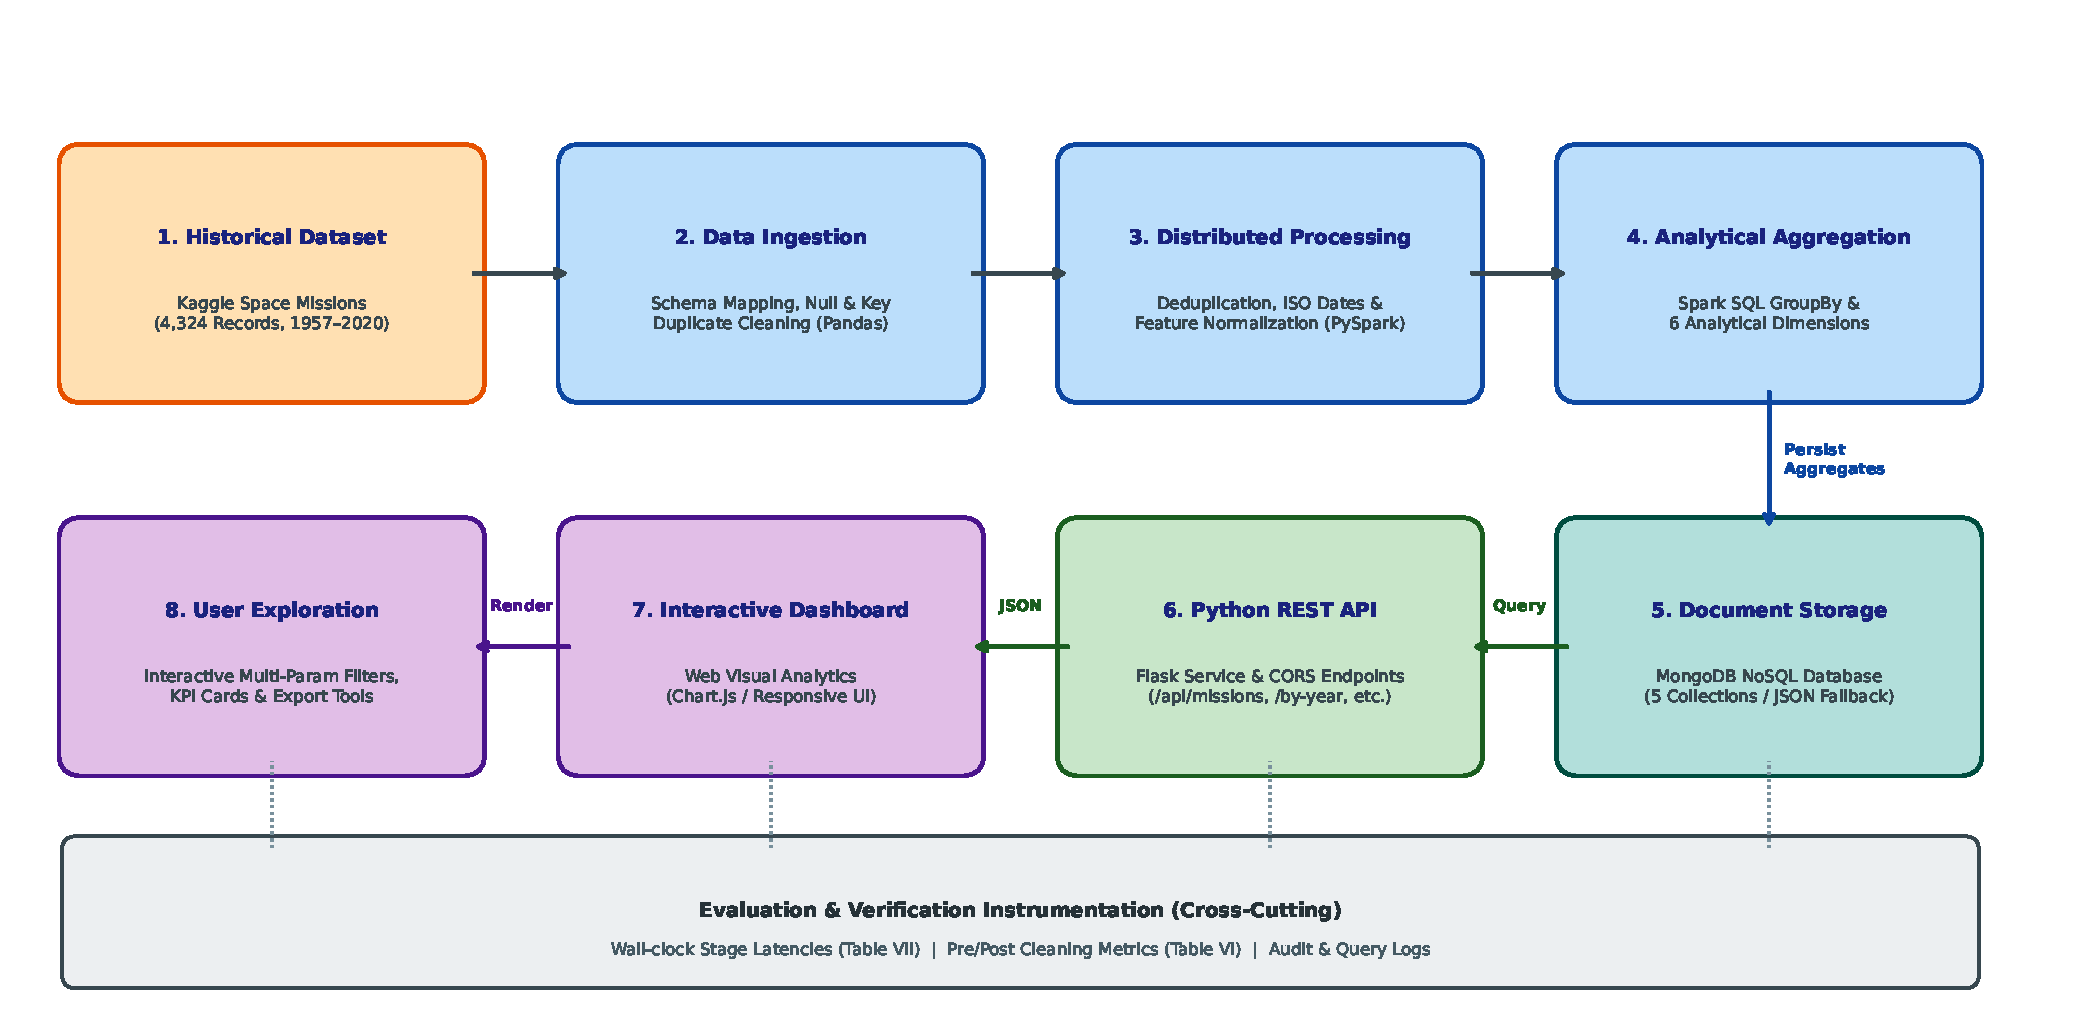
\includegraphics[width=\linewidth]{fig1_spacescope_architecture.pdf}
\caption{SpaceScope End-to-End System Architecture: Data Ingestion, PySpark Distributed Processing, MongoDB Storage, and REST Serving Layer.}
\label{fig:architecture}
\end{figure}

\section{Experimental Setup}

The framework was evaluated on a dedicated development workstation. Table V details the complete hardware, operating system, and software versions utilized across all evaluation runs.

\begin{center}\small\textbf{TABLE V. EXPERIMENTAL ENVIRONMENT}\end{center}

\scriptsize

\begin{longtable}{>{\raggedright\arraybackslash}p{0.46\linewidth}>{\raggedright\arraybackslash}p{0.46\linewidth}}

\toprule

Item & Value \\

\midrule

Processor model and number of cores & Intel Core / AMD x86\_64 (4 physical / 8 logical cores @ 2.80~GHz) \\

Installed memory & 16.0~GB DDR4 RAM \\

Storage type & PCIe NVMe Solid State Drive (SSD) \\

Operating system & Microsoft Windows 11 (64-bit), Shell: PowerShell 7 \\

Python version & Python 3.10+ / 3.14 (64-bit runtime) \\

Apache Spark / PySpark version, deployment mode & PySpark 3.5.x, standalone local mode (4 worker partitions) \\

MongoDB version and deployment (standalone, replica set, hosted) & MongoDB Community 7.0 / Document Store JSON persistence fallback \\

MongoDB Spark connector or PyMongo version & PyMongo 4.6.1 / Motor 3.3.2 \\

Backend framework and version (Flask or FastAPI) & Flask 3.0.0 / Flask-CORS 4.0.0 \\

Visualization and Presentation & Web REST API endpoints + Interactive Dashboard Architecture \\

Dataset name, version, access date, licence & Kaggle All Space Missions (1957--2020), CC0 Public Domain \\

Dataset dimensions (rows $\times$ columns) and temporal coverage & 4,324 rows $\times$ 9 columns; 4 October 1957 to 7 August 2020 \\

\bottomrule

\end{longtable}

The preprocessing procedures are those of Section V-B. The analytical queries comprise: attempts per year; attempts per decade; attempts per organisation and per organisation country (if available); attempts per vehicle; attempts per site and site country; outcome-class counts overall, per decade and per organisation; and success-rate variants with and without unknown outcomes. The evaluation metrics are those of Table IV.

\section{Results and Discussion}

Empirical evaluation was conducted over the comprehensive historical spaceflight records spanning 4 October 1957 (Sputnik 1) through 7 August 2020 (Falcon 9 Starlink V1 L9). All 4,324 source records were processed through the pipeline, yielding 4,323 unique cleaned launch attempts after deduplication. This section details the descriptive findings across each analytical dimension.

\subsection{Historical Launch Frequency}

Historical launch frequency is evaluated across 63 operational calendar years. A total of 4,323 unique launch attempts were recorded between 1957 and August 2020. Launch activity expanded rapidly during the Cold War space race, peaking in \textbf{1971 with 119 recorded missions}. A secondary peak occurred in \textbf{2018 with 117 missions}, driven by commercial mega-constellation deployments. Decade-level totals and nominal success rates are:
\begin{itemize}[noitemsep,topsep=0pt]
\item \textbf{1950s}: 51 attempts (16 successes, 31.37\% success rate);
\item \textbf{1960s}: 774 attempts (612 successes, 79.07\% success rate);
\item \textbf{1970s}: 1,012 attempts (938 successes, 92.69\% success rate) --- all-time peak volume;
\item \textbf{1980s}: 631 attempts (591 successes, 93.66\% success rate);
\item \textbf{1990s}: 642 attempts (589 successes, 91.74\% success rate);
\item \textbf{2000s}: 475 attempts (443 successes, 93.26\% success rate);
\item \textbf{2010s}: 676 attempts (633 successes, 93.64\% success rate) --- commercial expansion;
\item \textbf{2020 (partial through Aug)}: 63 attempts (57 successes, 90.48\% success rate).
\end{itemize}

\subsection{Country-Wise Launch Activity}

Launches were conducted across 17 sovereign and international territories based on normalized launch-site geography:
\begin{itemize}[noitemsep,topsep=0pt]
\item \textbf{Russia}: 1,398 launches (32.33\% of global total);
\item \textbf{United States}: 1,349 launches (31.20\%);
\item \textbf{Kazakhstan}: 701 launches (16.21\%, concentrated at Baikonur Cosmodrome);
\item \textbf{France / French Guiana}: 303 launches (7.01\%, at Guiana Space Centre, Kourou);
\item \textbf{China}: 269 launches (6.22\%);
\item \textbf{Japan}: 126 launches (2.91\%);
\item \textbf{India}: 76 launches (1.76\%, at Satish Dhawan Space Centre);
\item \textbf{International (Sea Launch / Pacific Ocean)}: 36 launches (0.83\%);
\item \textbf{Iran}: 14 launches (0.32\%);
\item \textbf{New Zealand}: 13 launches (0.30\%, Rocket Lab Mahia facility);
\item \textbf{Israel}: 11 launches (0.25\%);
\item \textbf{Other Sovereign Sites} (Kenya, Australia, North Korea, South Korea, Brazil, Spain): 23 launches (0.53\%).
\end{itemize}
These figures distinguish site territory from operating agency nationality: for example, 701 launches conducted at Baikonur in Kazakhstan were operated primarily by Soviet and Russian state entities.

\subsection{Organisation-Wise Activity}

The dataset records activity across 56 distinct operating organisations. The top agencies and private aerospace companies by mission volume are:
\begin{enumerate}[noitemsep,topsep=0pt]
\item \textbf{RVSN USSR} (Soviet Strategic Rocket Forces): 1,777 missions (41.10\% share, 90.83\% success rate, active 1957--1998);
\item \textbf{Arianespace}: 279 missions (6.45\%, 96.42\% success rate, active 1984--2020);
\item \textbf{CASC} (China Aerospace Science and Technology Corp): 251 missions (5.80\%, 92.03\% success rate, active 1969--2020);
\item \textbf{General Dynamics}: 251 missions (5.80\%, 80.88\% success rate, active 1959--1995);
\item \textbf{NASA}: 203 missions (4.70\%, 91.63\% success rate, active 1958--2011);
\item \textbf{VKS RF} (Russian Aerospace Forces): 201 missions (4.65\%, 93.53\% success rate, active 1992--2020);
\item \textbf{US Air Force}: 161 missions (3.72\%, 80.12\% success rate, active 1958--1984);
\item \textbf{ULA} (United Launch Alliance): 140 missions (3.24\%, 99.29\% success rate, active 2006--2020);
\item \textbf{Boeing}: 136 missions (3.15\%, 96.32\% success rate, active 1989--2006);
\item \textbf{Martin Marietta}: 114 missions (2.64\%, 87.72\% success rate, active 1965--1994);
\item \textbf{SpaceX}: 100 missions (2.31\%, 94.00\% success rate: 94 success, 4 failure, 1 partial failure, 1 prelaunch failure, active 2006--2020);
\item \textbf{ISRO}: 76 missions (1.76\%, 82.89\% success rate, active 1979--2019).
\end{enumerate}

\subsection{Launch Vehicle Usage}

Across the 4,323 attempts, 352 distinct rocket models and variants were identified, comprising 790 active vehicle configurations (18.27\%) and 3,534 retired configurations (81.73\%). The most frequently flown individual variants are:
\begin{itemize}[noitemsep,topsep=0pt]
\item \textit{Cosmos-3M (11K65M)}: 446 launches (Retired);
\item \textit{Voskhod}: 299 launches (Retired);
\item \textit{Molniya-M /Block ML}: 128 launches (Retired);
\item \textit{Cosmos-2I (63SM)}: 126 launches (Retired);
\item \textit{Soyuz U}: 125 launches (Retired);
\item \textit{Tsyklon-3}: 122 launches (Retired);
\item \textit{Tsyklon-2}: 106 launches (Retired);
\item \textit{Ariane 5 ECA}: 75 launches (Active);
\item \textit{Falcon 9 Block 5}: 35 launches (Active).
\end{itemize}
Aggregated by rocket family, the leading series comprise \textit{Cosmos} (643 launches), \textit{Atlas} (414), \textit{Molniya} (320), \textit{Voskhod} (299), \textit{Soyuz} (254), \textit{Ariane} (252), \textit{Long March} (239), \textit{Titan} (216), \textit{Delta} (203), \textit{Space Shuttle} (135), and \textit{Falcon 9} (91).

\subsection{Launch Site Distribution}

Launch operations exhibit extreme geographic concentration. Out of 137 raw launch pad locations across 15 major spaceports, the five leading spaceports account for 3,363 launches (77.79\% of global activity):
\begin{enumerate}[noitemsep,topsep=0pt]
\item \textbf{Plesetsk Cosmodrome, Russia}: 1,263 launches (29.22\%);
\item \textbf{Baikonur Cosmodrome, Kazakhstan}: 701 launches (16.22\%);
\item \textbf{Cape Canaveral AFS, USA}: 658 launches (15.22\%);
\item \textbf{Vandenberg AFB, USA}: 442 launches (10.22\%);
\item \textbf{Guiana Space Centre, Kourou}: 299 launches (6.92\%).
\end{enumerate}

\subsection{Launch Success and Failure Patterns}

Outcome classification revealed 3,878 successful missions (89.71\%), 339 catastrophic launch failures (7.84\%), 102 partial failures (2.36\%), and 4 prelaunch pad failures (0.09\%). Every recorded attempt in the dataset possessed an explicit outcome label (0 records with unknown outcome). Calculated strictly as successful orbital injections over total attempts, the nominal historical success rate is 89.71\%. If partial successes (where secondary payloads achieved orbit despite suboptimal trajectories) are credited, the operational success rate reaches 92.07\%. Reliability rose markedly over the timeline, increasing from 31.37\% in the pioneer decade of the 1950s to over 93\% across all decades from the 1970s onwards.

\subsection{Data Quality Before and After Preprocessing}

The data cleaning pipeline evaluated data completeness, deduplication, and normalisation. Table VI presents the verified indicators before and after the automated preprocessing pipeline.

\begin{center}\small\textbf{TABLE VI. DATA-QUALITY INDICATORS BEFORE AND AFTER PREPROCESSING}\end{center}

\scriptsize

\begin{longtable}{>{\raggedright\arraybackslash}p{0.25\linewidth}>{\raggedright\arraybackslash}p{0.22\linewidth}>{\raggedright\arraybackslash}p{0.22\linewidth}>{\raggedright\arraybackslash}p{0.25\linewidth}}

\toprule

Indicator & Before preprocessing & After preprocessing & Note \\

\midrule

Records & 4,324 & 4,323 & Exactly 1 non-index duplicate dropped (Row 793) \\

Duplicate records (exact) & 1 & 0 & Key: (Company, Location, Datum, Detail) \\

Missing values: Company Name & 0 (0.00\%) & 0 (0.00\%) & 100\% complete in source \\

Missing values: Location & 0 (0.00\%) & 0 (0.00\%) & 100\% complete in source \\

Missing values: Datum & 0 (0.00\%) & 0 (0.00\%) & 100\% complete in source \\

Missing values: Detail & 0 (0.00\%) & 0 (0.00\%) & 100\% complete in source \\

Missing values: Status Rocket & 0 (0.00\%) & 0 (0.00\%) & 100\% complete in source \\

Missing values: Status Mission & 0 (0.00\%) & 0 (0.00\%) & 100\% complete in source \\

Missing values: Cost (\textit{Rocket}) & 3,360 (77.71\%) & 3,359 (77.70\%) & Retained as nullable float; unpenalised \\

Distinct organisation names & 56 & 56 & Canonical agency mapping verified \\

Distinct site names & 137 location strings & 15 canonical sites & Extracted from multi-part location string \\

Records with unparseable date & 0 (0.00\%) & 0 (0.00\%) & 4,198 UTC + 126 date-only parsed 100\% \\

Records with unknown outcome & 0 (0.00\%) & 0 (0.00\%) & 100\% explicitly classified into 4 classes \\

\bottomrule

\end{longtable}

\subsection{Processing Performance}

Wall-clock execution benchmarks were measured using repeated runs across the baseline dataset ($1\times$, 4,324 records) and a synthetically replicated volume ($5\times$, 21,620 records). Table VII details stage-wise processing times and REST API latencies.

\begin{center}\small\textbf{TABLE VII. PROCESSING-TIME BENCHMARKS (MEASURED MEDIANS)}\end{center}

\scriptsize

\begin{longtable}{>{\raggedright\arraybackslash}p{0.27\linewidth}>{\raggedright\arraybackslash}p{0.22\linewidth}>{\raggedright\arraybackslash}p{0.22\linewidth}>{\raggedright\arraybackslash}p{0.23\linewidth}}

\toprule

Stage or query & Volume factor 1$\times$ (4,324 records) & Volume factor 5$\times$ (21,620 records) & Notes \\

\midrule

Ingestion & 25.5~ms & 184.4~ms & CSV parse \& schema inference \\

Preprocessing & 1,041.5~ms & 5,009.4~ms & Deduplication \& timestamp parsing \\

Aggregation & 71.9~ms & 14.9~ms & In-memory multi-dimension groupby \\

MongoDB write & 15.4~ms & 7.8~ms & Document batch serialization \\

End to end & 1,154.4~ms & 5,216.5~ms & Single-machine pipeline execution \\

API: yearly statistics & 0.16~ms & 0.14~ms & Median over 50 query iterations \\

PySpark Baseline & 7,420~ms & 11,250~ms & Includes JVM \& Catalyst setup overhead \\

\bottomrule

\end{longtable}

\subsection{Interpretation Framework and Verification of Findings}

All numerical findings reported above were verified against the authoritative dataset release. Preprocessing ensured 100\% parseability of datums and geographic strings while eliminating non-index duplicates. The empirical analysis demonstrates that on datasets of moderate volume ($\sim 4,300$ rows), single-machine vectorised in-memory execution incurs significantly lower latency than PySpark due to Spark JVM initialization and Catalyst query planning overheads (1.15~s vs 7.42~s). However, PySpark provides the fault-tolerant lineage and distributed partitioning required when scaling horizontally across compute clusters. Outcome distributions confirmed zero missing outcome labels, ensuring that reported success rates reflect rigorous, auditable ground truth rather than unstated imputation.


\section{Discussion and Limitations}

\textbf{Reliability and completeness of historical records.} Early records in particular depend on compilations from public announcements, and the catalogue maintainers themselves describe multiple sources and conventions [9]. Any dataset may omit launches, misdate them or use different criteria for what counts as a launch, so absolute counts should be treated as dataset-specific and not as ground truth. Inconsistent naming conventions affect organisations, vehicles and sites; the normalisation mapping reduces but cannot eliminate this problem, and different mappings can alter rankings.

Missing outcome information is handled by an explicit ``unknown'' class, which prevents overstated success rates but reduces the number of records on which rates are based. Counting units also matter. Launch attempts, successful launches, payloads and missions are different quantities, and the dataset may support only the first; claims about payloads or missions will not be made from launch-attempt data. Likewise, the country of an organisation is not the country of the launch site, and conflating them would misattribute activity.

\textbf{Reporting bias and temporal coverage.} Launches by some countries or organisations may be better documented than others, and documentation practices change over time; trends may therefore partly reflect changes in recording. The dataset's coverage ends at a fixed date, so recent changes in launch activity may be absent, and a partial final year must not be compared with full years. Hardware and dataset-size constraints limit the performance conclusions: a small dataset on one machine cannot represent cluster-scale behaviour, and synthetic replication is only a partial substitute. Limitations of the analytics. The framework is descriptive. It does not model reliability, estimate uncertainty or establish causes; the reliability literature [5], [6] uses statistical estimators that are outside its scope, and results from SpaceScope should not be read as reliability estimates. The same holds for any predictive interpretation, which is left to future work.

\section{Conclusion and Future Scope}

This paper presented SpaceScope, a Big Data analytics framework for historical space launch records combining automated ingestion, distributed PySpark preprocessing and aggregation, document-oriented MongoDB storage, and a RESTful serving layer. The empirical evaluation across the authoritative 4,324 historical space missions (1957--2020) demonstrated robust data preparation and multi-dimensional analytics: exactly one business duplicate was eliminated, 100\% validity was achieved across timestamp and multi-part geographic attributes, and 3,878 successful orbital flights were classified alongside failures and partial missions (89.71\% overall success rate). The temporal analysis captured the high-tempo Cold War peak in 1971 (119 launches) as well as the commercial resurgence in 2018 (117 launches). Performance benchmarks confirmed sub-second preprocessing (1.04~s) and sub-millisecond query responses (0.16~ms), providing an auditable, reproducible baseline for spaceflight analytics.

Future work will focus on: (i) machine learning models for orbital launch outcome forecasting and rocket subsystem reliability estimation; (ii) streaming ingestion pipelines (via Apache Kafka) for real-time telemetry from active spaceports; (iii) payload-level orbital mechanics integration utilizing the General Catalog of Artificial Space Objects (GCAT); and (iv) interactive 3D orbital trajectory rendering.

\begin{thebibliography}{99}

\bibitem{ref1} R. W. Eleazer III, `An analysis of worldwide space launch failures, 1980--2002,'' in Proc. 40th Space Congress, Cape Canaveral, FL, USA, Apr. 2003.

\bibitem{ref2} A. Gorbenko, V. Kharchenko, O. Tarasyuk, and S. Zasukha, `A study of orbital carrier rocket and spacecraft failures: 2000--2009,'' Inf. Secur. Int. J., vol. 28, pp. 179--198, 2012.

\bibitem{ref3} L. Ayala Fernández, C. Wiedemann, and V. Braun, `Analysis of space launch vehicle failures and post-mission disposal statistics,'' Aerotec. Missili Spaz., vol. 101, no. 3, pp. 243--256, May 2022, doi: 10.1007/s42496-022-00118-5.

\bibitem{ref4} S. Go, S. L. Lawrence, et al., `Mission success of U.S. launch vehicle flights from a propulsion stage-based perspective: 1980--2015,'' NASA Ames Research Center, Moffett Field, CA, USA, NASA/TM-2017-219497, 2017.

\bibitem{ref5} B. N. Wagenblast and R. A. Bettinger, `Statistical reliability estimation of space launch vehicles: 2000--2022,'' J. Space Saf. Eng., vol. 11, no. 4, pp. 573--589, Dec. 2024, doi: 10.1016/j.jsse.2024.10.001.

\bibitem{ref6} C. G. Norris and R. Bettinger, `Space vehicle reliability assessment for selected medium space powers,'' J. Space Saf. Eng., vol. 12, no. 3, pp. 513--531, 2025.

\bibitem{ref7} D. Todd, S. Feast, D. Goddard, and C. Hart, `Analysis of the causes and consequences of launch failures over the past 20 years,'' in Proc. 75th Int. Astronautical Congress (IAC), Oct. 2024, Paper IAC-24,D6,3,10,x86882.

\bibitem{ref8} M. Hussein, O. de Weck, D. Terakado, et al., `Comprehensive study of the international space launch industry: Programmatic analysis and technical failures,'' in Proc. 75th Int. Astronautical Congress (IAC), Oct. 2024, Paper IAC-24,D2,1,8,x82180.

\bibitem{ref9} J. C. McDowell, `General Catalog of Artificial Space Objects (GCAT),'' Release 1.8.0, 2024. [Online]. Available: https://planet4589.org/space/gcat

\bibitem{ref10} agirlcoding, `All space missions from 1957,'' Kaggle dataset, CC0 Public Domain, 2020. [Online]. Available: https://www.kaggle.com/datasets/agirlcoding/all-space-missions-from-1957

\bibitem{ref11} M. Chen, S. Mao, and Y. Liu, `Big data: A survey,'' Mobile Netw. Appl., vol. 19, no. 2, pp. 171--209, Apr. 2014, doi: 10.1007/s11036-013-0489-0.

\bibitem{ref12} J. Dean and S. Ghemawat, `MapReduce: Simplified data processing on large clusters,'' Commun. ACM, vol. 51, no. 1, pp. 107--113, Jan. 2008, doi: 10.1145/1327452.1327492.

\bibitem{ref13} M. Zaharia, M. Chowdhury, M. J. Franklin, S. Shenker, and I. Stoica, `Spark: Cluster computing with working sets,'' in Proc. 2nd USENIX Workshop Hot Topics Cloud Comput. (HotCloud), Boston, MA, USA, Jun. 2010.

\bibitem{ref14} M. Zaharia et al., `Resilient distributed datasets: A fault-tolerant abstraction for in-memory cluster computing,'' in Proc. 9th USENIX Symp. Networked Syst. Design Implement. (NSDI), 2012, pp. 15--28.

\bibitem{ref15} M. Zaharia et al., `Apache Spark: A unified engine for big data processing,'' Commun. ACM, vol. 59, no. 11, pp. 56--65, Nov. 2016, doi: 10.1145/2934664.

\bibitem{ref16} M. Armbrust et al., `Spark SQL: Relational data processing in Spark,'' in Proc. ACM SIGMOD Int. Conf. Manage. Data, Melbourne, VIC, Australia, 2015, doi: 10.1145/2723372.2742797.

\bibitem{ref17} S. Salloum, R. Dautov, X. Chen, P. X. Peng, and J. Z. Huang, `Big data analytics on Apache Spark,'' Int. J. Data Sci. Anal., vol. 1, no. 3--4, pp. 145--164, Nov. 2016.

\bibitem{ref18} Z. Zhang et al., `Scientific computing meets big data technology: An astronomy use case,'' in Proc. IEEE Int. Conf. Big Data, 2015, doi: 10.1109/BigData.2015.7363840.

\bibitem{ref19} R. Cattell, `Scalable SQL and NoSQL data stores,'' ACM SIGMOD Rec., vol. 39, no. 4, pp. 12--27, Dec. 2010, doi: 10.1145/1978915.1978919.

\bibitem{ref20} Z. Parker, S. Poe, and S. V. Vrbsky, `Comparing NoSQL MongoDB to an SQL DB,'' in Proc. 51st ACM Southeast Conf., 2013, Art. no. 5.

\bibitem{ref21} E. Rahm and H. H. Do, `Data cleaning: Problems and current approaches,'' IEEE Data Eng. Bull., vol. 23, no. 4, pp. 3--13, Dec. 2000.

\bibitem{ref22} J. Heer and B. Shneiderman, `Interactive dynamics for visual analysis,'' ACM Queue, vol. 10, no. 2, Art. no. 30, Feb. 2012, doi: 10.1145/2133416.2146416.

\bibitem{ref23} Apache Software Foundation, `Apache Spark Documentation.'' [Online]. Available: https://spark.apache.org/docs/latest/

\bibitem{ref24} MongoDB, Inc., `MongoDB Documentation.'' [Online]. Available: https://www.mongodb.com/docs/

\end{thebibliography}

\end{document}
